\section{Vectors}
\label{sec_vectors}

Example program which defines vector field {\tt uvw}, assigns initial
values to it, and plots it, is given below:
%
{\small \begin{verbatim}
     ...
     20   /* define unknowns */
     21   Vector uvw(d); // velocity
     22
     23   /* assign initial values to velocity in "i" direction */
     24   Comp m = Comp::u();
     25   for_vmijk(uvw,m,i,j,k)
     26     uvw[m][i][j][k] =  sin(uvw.xc(m,i)) * cos(uvw.yc(m,j)) * cos(uvw.zc(m,k));
     27
     28   /* assign initial values to velocity in "j" direction */
     29   Comp m = Comp::v();
     30   for_vmijk(uvw,m,i,j,k)
     31     uvw[m][i][j][k] = -cos(uvw.xc(m,i)) * sin(uvw.yc(m,j)) * cos(uvw.zc(m,k));
     32
     33   /* plot vector */
     34   boil::plot->plot(uvw, "velocity", 0);
     ...
\end{verbatim}}
%
Only the lines which are different to program {\tt 06-01-main.cpp} are given. This
program is stored as {\tt 06-03-main.cpp}. Velocity vector {\tt uvw} is created 
from computational domain only in line~21, as an object of type {\tt Vector}.

Vector field {\tt uvw} stores three Cartesian velocity components: $u$,
$v$ and $w$. The program actually initializes {\tt uvw} to:
%
\bea
  u & = &  sin(x) cos(y) cos(z) \\
  v & = & -cos(x) sin(y) cos(z) \\
  w & = & 0
  \label{eq_velocity}
\eea
%
Observe in lines~26 and~31 that {\tt Vector} fields are accessed like the 
four-dimensional matrices in {\tt C++}: {\tt uvw[m][i][j][k];}, where {\tt m} is 
a component counter ({\tt Comp::u()} for $u$, {\tt Comp::v()} for $v$ and 
{\tt Comp::w()} for $w$), and {\tt i}, {\tt j} 
and {\tt k} are positions in three-dimensional structured domain. 

For shorter and safer browsing through vectors, a number of macros have been
defined in {\tt Vector/vector\_browsing.h}, in a similar way it was done
for scalar. Two examples are given in above
listing, in lines~25 and~30. The macro:
%
{\small \begin{verbatim}
     30   for_vmijk(uvw,m,i,j,k)
\end{verbatim}}
%
takes as parameters the {\tt Vector} field ({\tt uvw}), the component for
which you want to browse ({\tt m}), and counters in $i$, $j$ and $k$ 
direction ({\tt i}, {\tt j} and {\tt k}.

One might wonder at this point why do we have to send vector component ({\tt m})
to macro for browsing, isn't the grid defined by {\tt Vector}'s member functions
{\tt si()}, {\tt ei()}, {\tt sj()}, \ldots. Well, it must not be forgotten that
vectors are defined on a staggered grid, which means their resolution is different
from {\tt Scalar}'s, and, even more, it is different for each vector component.

Make a small test. Insert the following lines to program~{\tt 06-03-main.cpp}:
%
{\small \begin{verbatim}
     33   /* resolution of "u" velocity component */
     34   OPR(uvw.ni( Comp::u() ));
     35   OPR(uvw.nj( Comp::u() ));
     36   OPR(uvw.nk( Comp::u() ));
     37   /* resolution of "v" velocity component */
     38   OPR(uvw.ni( Comp::v() ));
     39   OPR(uvw.nj( Comp::v() ));
     40   OPR(uvw.nk( Comp::v() ));
     41   /* resolution of "w" velocity component */
     42   OPR(uvw.ni( Comp::w() ));
     43   OPR(uvw.nj( Comp::w() ));
     44   OPR(uvw.nk( Comp::w() ));
\end{verbatim}}
%
Re-compile and re-run to get:
%
{\small \begin{verbatim}
FILE: main.cpp, LINE: 34, uvw.ni( Comp::u() ) = 67
FILE: main.cpp, LINE: 35, uvw.nj( Comp::u() ) = 66
FILE: main.cpp, LINE: 36, uvw.nk( Comp::u() ) = 66
FILE: main.cpp, LINE: 38, uvw.ni( Comp::v() ) = 66
FILE: main.cpp, LINE: 39, uvw.nj( Comp::v() ) = 67
FILE: main.cpp, LINE: 40, uvw.nk( Comp::v() ) = 66
FILE: main.cpp, LINE: 42, uvw.ni( Comp::w() ) = 66
FILE: main.cpp, LINE: 43, uvw.nj( Comp::w() ) = 66
FILE: main.cpp, LINE: 44, uvw.nk( Comp::w() ) = 67
\end{verbatim}}
%
Apparently, resolution is different for each vector component. The reason is
easy to understand. As the grid in shifted\footnote{staggered} in $i$ direction, 
additional cells are created on the plane of faces at the beginning of the domain. 
The same holds for shifts in $j$ and $k$ direction, with increase in according
directions.
The increase of number of cells due to staggering is illustrated 
in Fig.~\ref{fig_staggering}.
%
%--------------%
%              %
%  Staggering  %
%              %
%--------------%
\begin{figure}[ht]
  \centering
  \setlength{\unitlength}{1mm}
  \begin{picture}(100,50)(0,0)
    \thickbox{100}{50}
    \put(0,0){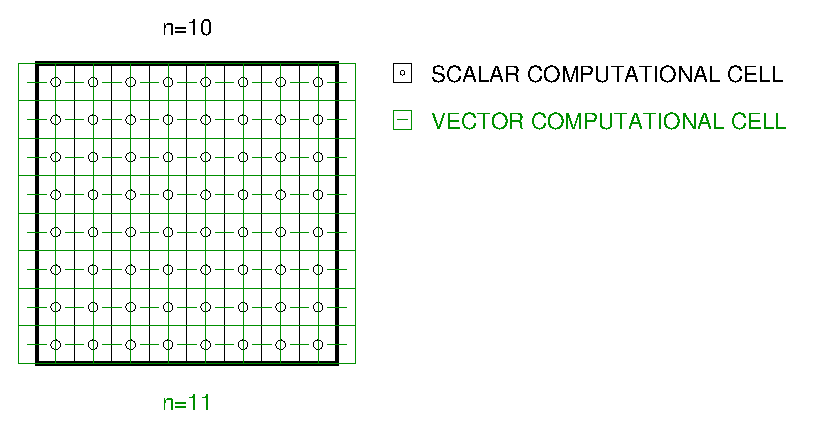
\includegraphics[scale=0.75]{Figures/06-02-staggering.eps}}
  \end{picture}
  \caption{Number of cell rows for a {\tt Vector} field is greater by
           one  than than for {\tt Scalar} field, in the direction
           of staggering.}
  \label{fig_staggering}
\end{figure}
%
For the same reason, many {\tt Vector}'s member functions related to geometrical 
quantities (such as {\tt dxc()}, {\tt dyc()}, {\tt dzc()}, {\tt dxw()}, {\tt dxe()},
{\tt dV()}, \ldots) also depend on {\tt Vector}'s component.

Velocity field prescribed by program ({\tt 06-03-main.cpp}) is shown in
Fig.~\ref{fig_velocity}.
 
%------------%
%            %
%  Velocity  %
%            %
%------------%
\begin{figure}[ht]
  \centering
  \setlength{\unitlength}{1mm}
  \begin{picture}(100,85)(0,0)
    \thickbox{100}{85}
    \put(0,-3){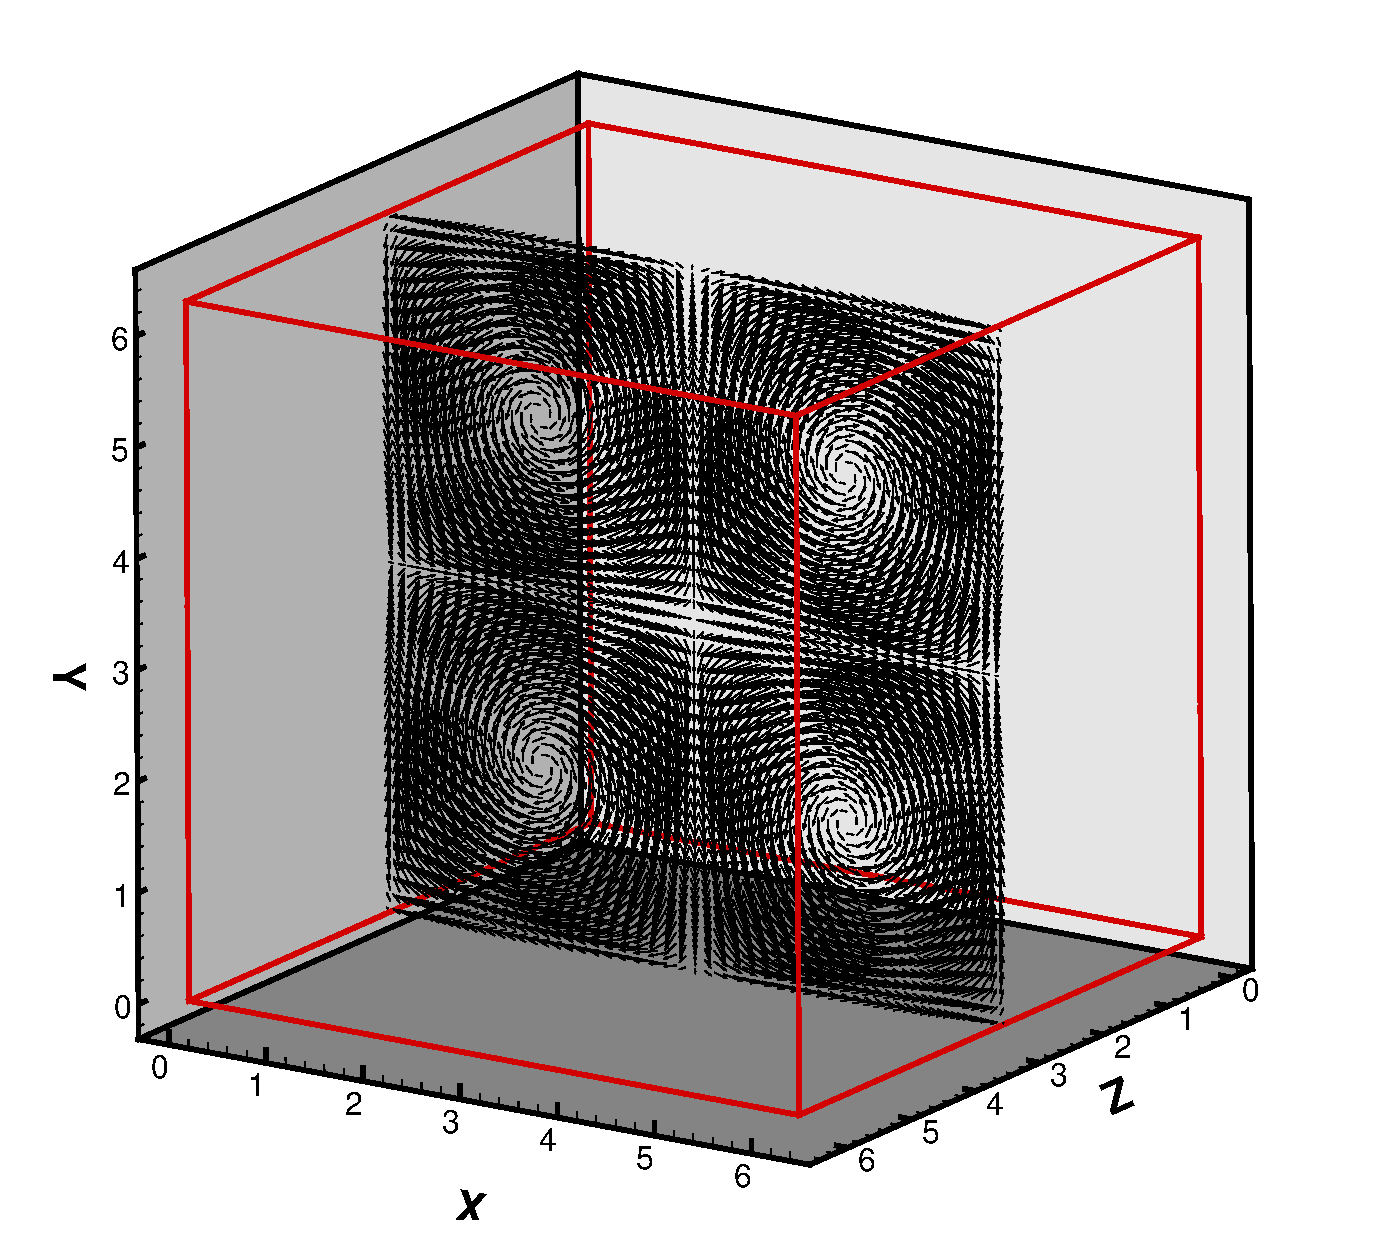
\includegraphics[scale=0.45]{Figures/06-03-velocity.eps}}
  \end{picture}
  \caption{Pressure field prescribed by Eq.~\ref{eq_velocity}}
  \label{fig_velocity}
\end{figure}

\clearpage

%---------------------------------------------------------------------nutshell-%
\vspace*{5mm} \fbox{ \begin{minipage}[c] {0.97\textwidth} %-----------nutshell-%
    {\sf Section \ref{sec_vectors} in a nutshell} \\  %---------------nutshell-%
   
      - Vector fields are defined with {\psiboil} class {\tt Vector}. \\

      - {\tt Vector} is defined for a {\tt Domain}, with the constructor:
      \begin{itemize}
        \item {\tt Vector(Domain \&);}
      \end{itemize}
 
      - {\tt Vector}'s values are accessed with the usual {\tt C++} syntax:
      \begin{itemize}
        \item {\tt p[m][i][j][k];}
      \end{itemize}
      where {\tt m} is a vector component ranging from 0-3 (for $i$, $j$ and $k$). \\

      - To browse through all the {\tt Vector} values of component {\tt m}, 
      use the following macro:
      \begin{itemize}
        \item {\tt for\_vmijk(Vector \&, int m, int i, int j, int k);}
      \end{itemize}
       Similar macros are defined in directory: {\tt PSI-Boil/Src/Vector/vector\_browsing}. \\

      - {\tt Vector} has a number of member functions to access {\tt Domain}s
      geometrical quantities. Most of them depend on the {\tt Vector}'s component
    
  \end{minipage} } %--------------------------------------------------nutshell-%
%---------------------------------------------------------------------nutshell-%
